\documentclass[12pt]{article}
\usepackage[margin=1.5cm]{geometry}
\usepackage{parskip}
\usepackage{amsmath}
\usepackage{amssymb}
\usepackage{amsfonts}
\usepackage{enumitem}
\usepackage{graphicx}
\usepackage{stmaryrd}
\graphicspath{ {./images/} }


\begin{document}
\begin{enumerate}[label=(\alph*)]

  \item
    A variable is live at a particular program point if assigning that variable to a different value at that program point would cause the behaviour of the program to change in some observable way. This is a semantic notion of variable liveness, since we only consider real executions of the program. In terms of computing liveness, we use a syntactic version, which considers all possible program paths as viable, even if they are not, for example:

\begin{verbatim}
L0: x = 5
if ((x+1) * (x+1) == 0) {
  x = 0
}
if (x*x + 2*x + 1 != 0) {
  x = 1
}
print x
\end{verbatim}

In this code, $x$ would not be semantically live at L0, since it will always get assigned to 0 or 1, but this is uncomputable in general, so we treat it as syntactically live at L0.

An algorithm to compute liveness comes from the following data-flow equation:

\[
  live(n) = \left(\bigcup_{s \in succ(n)} live(s)\right) \setminus kill(n) \cup gen(n)
\] 

Where $kill(n)$ is the set of variables killed (defined) at $n$, and $gen(n)$ is the set of variables generated (referenced) at $n$.

An algorithm would look like the following:

\begin{verbatim}
for i=1 to n do live[i] = {}
while (live[] changes)
  for i=n to 1 do
    live[i] = big_union(s in succ(n), live[s]) \ kill(n) U gen(n)
\end{verbatim}

\item
  Live variable sets are given below:
\begin{verbatim}
L0: {q}
L1: {p,q}
L2: {p,q}
L3: {p,q,v}
L4: {p,q,v}
L5: {p,q,t}
L6: {t}
L7: {p,q,t}
L8: {p,q}
\end{verbatim}

Here, we over-approximate that \texttt{q} is live at L0 and L1, since on the first iteration, \texttt{p} is always 0, so \texttt{q} is always initialised.

\item
  This code does have a data-flow anomaly: the variable \texttt{q} is live at its declaration (or entry), meaning that it is used before it is defined, so a helpful compiler would alert the programmer that variable \texttt{q} is used before it is defined.

\item
  From our live variable sets, we construct the following clash graph:

  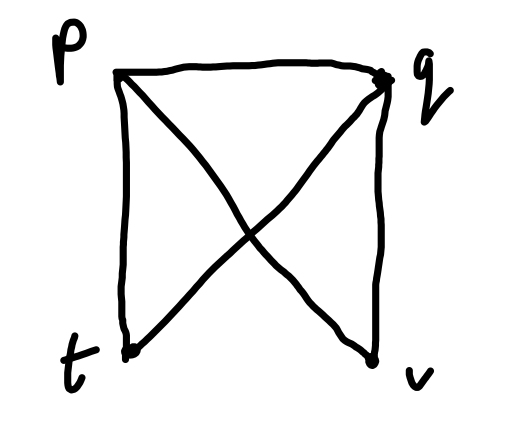
\includegraphics[scale=0.3]{clashgraph}

  Since \texttt{t} and \texttt{v} are not live together, a register allocator would likely allocate them to the same register. Ideally, this would be register \texttt{r0}, since they are not live over the function call to \texttt{readint()}, and in the function call to \texttt{cons}, \texttt{v} needs to be in register \texttt{r0} anyway.

  Since \texttt{p} and \texttt{q} are live over a procedure call (and clash with all other variables), we must allocate them to unique registers from \texttt{r4}, \texttt{r5}, \texttt{r6}, \texttt{r7}, the choice of which is arbitrary. Assuming we only have the 8 registers available to us, this requires a spill to memory in order to adhere to the ABI and preserve those registers.

  It would be wrong to simply allocate \texttt{p,q,t,v} to \texttt{r5,r6,r7,r8}, because this would require extra memory accesses to adhere to the ABI, as well as extra instructions to move parameters into \texttt{r0} (for \texttt{v}), and move results out (for \texttt{t} and \texttt{v}).

\item
  An allocator would have to spill certain registers to memory, e.g. on the stack frame.

  One solution to the source code would be to add an extra line before L2 (and after L1):

  \texttt{q = 0}

  This assignment to \texttt{q} means that \texttt{q} would not be live for L0 and L1, and so we could utilise an extra register in the complex code in L1, which means we would not have to spill to memory.



        
    \end{enumerate}
\end{document}
